% Generated by book/tools/notebook_to_tex.py. Do not edit by hand.

\chapter[DPO 정렬 (Preference Alignment)]{DPO: 사람 선호로 정렬 (Preference Alignment)}

\label{ch:30}

\markboth{DPO 정렬 (Preference Alignment)}{DPO 정렬 (Preference Alignment)}

\chaptermeta{30_dpo/30_dpo.ipynb}{https://colab.research.google.com/github/yoon-gu/neuqes-101/blob/master/30_dpo/30_dpo.ipynb}{reward model 없이 preference 쌍으로 policy를 직접 정렬하는 DPO 학습 단계를 정리}



\index{1DPO@DPO}

\index{1Direct Preference Optimization@Direct Preference Optimization}

\index{1preference alignment@preference alignment}

\index{1alignment@alignment}

\index{1chosen@chosen}

\index{1rejected@rejected}

\index{1reward margin@reward margin}

\index{1implicit reward@implicit reward}

\index{1reference model@reference model}

\index{1frozen reference@frozen reference}

\index{1KL constraint@KL constraint}

\index{1DPOTrainer@DPOTrainer}

\index{1DPOConfig@DPOConfig}

\index{1beta@beta}

\index{1RLAIF@RLAIF}

\index{1UltraFeedback@UltraFeedback}

\index{1maywell ko Ultrafeedback binarized@maywell/ko\_Ultrafeedback\_binarized}

\index{1policy model@policy model}

\index{1PPO@PPO}

\index{1reward model@reward model}

\index{1labels 100@labels=-100}

\index{1response only@response-only}

\index{0사람 선호@사람 선호}

\index{0선호 정렬@선호 정렬}

\index{0정렬 학습@정렬 학습}

\index{0선택 응답@선택 응답}

\index{0거절 응답@거절 응답}

\index{0보상 마진@보상 마진}

\index{0참조 모델@참조 모델}

\index{0고정 참조@고정 참조}

\index{0KL 제약@KL 제약}

\index{0응답 구간 손실@응답 구간 손실}

\index{1DPO loss@DPO loss}

\index{1margin 0@margin=0}

\index{1loss 0 6931@loss=0.6931}

\index{1sigmoid loss@sigmoid loss}

\index{1policy@policy}

\index{1frozen ref@frozen ref}

\index{1ref model None@ref\_model=None}

\index{1completion only preference@completion-only preference}

\index{1instruction following@instruction-following}

\index{1truthfulness@truthfulness}

\index{1honesty@honesty}

\index{1helpfulness@helpfulness}

\index{1binarized preference@binarized preference}

\index{1GPT 4 judge@GPT-4 judge}

\index{1PPO 4 models@PPO 4 models}

\index{1T4 training@T4 training}

\index{1gradient accumulation steps@gradient\_accumulation\_steps}

\index{1fp16@fp16}

\index{1reward accuracy@reward accuracy}

\index{1DPO beta@DPO beta}

\index{0선호 쌍@선호 쌍}

\index{0마진 직관@마진 직관}

\index{0기준 정책@기준 정책}

\index{0정책 최적화@정책 최적화}

\index{0품질 정렬@품질 정렬}

\index{0정직성@정직성}

\index{0유용성@유용성}

\index{0사실성@사실성}

\index{0지시 준수@지시 준수}

\index{0이진화 선호@이진화 선호}



\section{누적 추적표}

\begin{booktable}{30장 누적 추적표 표}{tab:ch30-01}
\begin{adjustbox}{max width=\textwidth}
\begin{tabular}{@{}llllll@{}}
\toprule
Ch & 모델 & 데이터 & 학습 신호 & Loss & Trainer \\
\midrule

27 & KoGPT2 (125M) & 한국어 TinyStories 30K & next-token & \inlinecode{CrossEntropyLoss} - continual pretraining & \inlinecode{Trainer} \\
28 & KoGPT2 (125M, SFT) & KoAlpaca instruction-response 쌍 & response 토큰 (답변만) & \inlinecode{CrossEntropyLoss} (response-only) - SFT & \inlinecode{SFTTrainer} \\
29 & \ref{ch:28}장 SFT 모델 (평가) & 분야별 벤치마크 & - (평가만) & - (\inlinecode{lm-evaluation-harness}) & - \\
\textbf{30 \(\leftarrow\) 여기} & \textbf{SFT 모델 (policy) + frozen reference} & \textbf{preference 쌍 (chosen / rejected)} & \textbf{chosen 선호 ↑ / rejected 선호 \(\downarrow\)} & \textbf{DPO sigmoid loss (\(\beta\)=0.1)} & \textbf{\inlinecode{DPOTrainer}} \\
31 (다음) & SFT 모델 + verifier & verifiable-reward prompts (수학·코드) & group relative advantage & \inlinecode{GRPO\ loss} & \inlinecode{GRPOTrainer} \\
\bottomrule
\end{tabular}
\end{adjustbox}
\end{booktable}

전체 장 표는 \href{https://github.com/yoon-gu/neuqes-101\#챕터별-변화추적표}{루트 README} 를 참고하세요.

\begin{center}\rule{0.5\linewidth}{0.5pt}\end{center}

\section{GPT 시대 학습 4단계 --- 본 장의 위치 (단계 4, Alignment / DPO)}

\ref{ch:24}장에서 도입한 GPT 시대 학습 4단계 표. 본 장은 \emph{단계 4 (Alignment)} --- \emph{사람의 선호에 맞춰 정렬} 하는 마지막 단계의 첫 방식 (DPO) 입니다.

\begin{booktable}{30장 GPT 시대 학습 4단계 - 본 장의 위치 (단계 4, Alignment / DPO) 표}{tab:ch30-02}
\begin{adjustbox}{max width=\textwidth}
\begin{tabular}{@{}llllll@{}}
\toprule
단계 & 정확 용어 & 의미 & 학습 신호 & 본 커리큘럼 & 본 장? \\
\midrule

1 & \textbf{Pretraining} (사전학습) & random init 본체 + 일반 코퍼스 & next-token & \ref{ch:24}장 (영어), \ref{ch:26}장 (한국어) & \\
2 & \textbf{Continual pretraining} (계속 사전학습) & 사전학습 본체 + 새 데이터 & next-token & \ref{ch:25}장 (영어), \ref{ch:27}장 (한국어) & \\
3 & \textbf{SFT} (Supervised Fine-Tuning) & instruction-response 로 \emph{행동 정렬} & response 토큰 & \ref{ch:28}장 & \\
4 & \textbf{Alignment} (DPO / RLHF / GRPO) & preference·verifier reward 로 \emph{선호 정렬} & preference 쌍 / reward & \textbf{\ref{ch:30}장 (DPO) \(\leftarrow\) 여기}, \ref{ch:31}장 (GRPO) & OK \\
\bottomrule
\end{tabular}
\end{adjustbox}
\end{booktable}

\subsection{\texorpdfstring{단계 3 (SFT) \(\to\) 단계 4 (Alignment) 의 결정적 변화}{단계 3 (SFT) \textbackslash to 단계 4 (Alignment) 의 결정적 변화}}

\begin{itemize}
\tightlist
\item
  \textbf{단계 3 (SFT)}: \emph{“좋은 답변 하나”} 를 따라 학습 (정답 demonstration 모방). 모델은 \emph{지시를 따르는 법} 을 배웁니다 --- 하지만 \emph{“여러 답변 중 어느 게 더 나은가”} 라는 \emph{선호} 는 가르치지 못합니다
\item
  \textbf{단계 4 (Alignment / DPO)}: \emph{“같은 질문에 좋은 답 vs 나쁜 답”} 쌍으로 학습. 모델은 \emph{사람이 선호하는 방향} 으로 정렬됩니다 --- \emph{더 도움되고, 더 안전하고, 더 품질 높은} 답 쪽으로
\end{itemize}

\begin{quote}
SFT 가 \emph{지시를 따르게} 했다면, alignment 는 \emph{따르는 방식을 사람의 선호에 맞춥니다}. DPO 는 그 alignment 를 \emph{reward model 없이, preference 쌍으로 직접} 해내는 방식입니다 --- RLHF (PPO) 의 간소화. 그 핵심은 아래 §4 의 DPO loss 한 줄입니다.
\end{quote}



\section{변경점 (Diff from \ref{ch:28}장 SFT)}

\begin{booktable}{30장 변경점 요약}{tab:ch30-03}
\begin{adjustbox}{max width=\textwidth}
\begin{tabular}{@{}lll@{}}
\toprule
축 & \ref{ch:28}장 (KoGPT2 SFT) & \ref{ch:30}장 (본 장, DPO) \\
\midrule

본체 & KoGPT2 \inlinecode{skt/kogpt2-base-v2} (125M) & \textbf{SFT 모델 (= KoGPT2 SFT 산출) 을 policy 로} \(\leftarrow\) 출발점이 SFT 모델 \\
토크나이저 & \inlinecode{PreTrainedTokenizerFast} (KoGPT2 BBPE) & \textbf{(동일)} \(\leftarrow\) 고정 \\
\textbf{데이터} & instruction-response 쌍 (\inlinecode{prompt} / \inlinecode{completion}) & \textbf{preference 쌍 (\inlinecode{prompt} / \inlinecode{chosen} / \inlinecode{rejected})} \(\leftarrow\) \emph{변화 1} \\
\textbf{Trainer} & \inlinecode{trl.SFTTrainer} & \textbf{\inlinecode{trl.DPOTrainer}} \(\leftarrow\) \emph{변화 2} (새 클래스, 첫 등장) \\
\textbf{Loss} & next-token \inlinecode{CrossEntropyLoss} (response-only) & \textbf{DPO sigmoid loss} \(\leftarrow\) \emph{변화 3} (log-likelihood ratio) \\
\textbf{reference 모델} & 없음 (policy 하나) & \textbf{frozen reference 추가} \(\leftarrow\) \emph{변화 4} (SFT 모델 복사 + freeze) \\
학습 신호 & 좋은 답변 하나 \emph{모방} & \textbf{chosen 선호 ↑, rejected 선호 \(\downarrow\)} (\emph{비교}) \\
lr & 2e-5 & \textbf{5e-6 - 1e-5} \(\leftarrow\) DPO 는 SFT 보다 작은 lr (reference 에서 천천히 벗어남) \\
\bottomrule
\end{tabular}
\end{adjustbox}
\end{booktable}

\begin{quote}
\textbf{핵심}: SFT 는 \emph{하나의 좋은 답} 을 모방했다면, DPO 는 \emph{(좋은 답, 나쁜 답) 쌍} 을 \emph{비교} 합니다. 그러려면 \emph{(1) preference 데이터}, \emph{(2) 비교를 loss 로 바꾸는 DPOTrainer}, \emph{(3) “원본에서 얼마나 벗어났나” 의 기준이 되는 frozen reference} 가 필요합니다. 네 가지가 한꺼번에 바뀌지만, \emph{목적은 하나} --- \emph{모델을 사람이 선호하는 방향으로} 정렬.
\end{quote}



\section{alignment 의 의미 --- SFT(지시 따름) 에서 선호·안전성·품질 정렬로}

\textbf{alignment (정렬)} 은 모델의 행동을 \emph{사람이 원하는 방향} 에 맞추는 단계입니다. SFT 와의 차이를 한 줄로:

\begin{itemize}
\tightlist
\item
  \textbf{SFT}: \emph{지시를 따르게} 만든다 (행동 정렬). “질문이 오면 답하라”
\item
  \textbf{Alignment}: \emph{따르는 방식을 사람의 선호에 맞춘다} (선호 정렬). “기왕 답할 거면, 더 도움되고·안전하고·품질 높게”
\end{itemize}

\subsection{RLHF 흐름 --- 그리고 DPO 가 그 간소화인 이유}

전통적인 \textbf{RLHF (Reinforcement Learning from Human Feedback)} 는 세 단계입니다:

\Needspace{5\baselineskip}
\begin{lstlisting}
1. SFT          : instruction-response 로 base 모델을 지시 따르게 (28장)
2. Reward Model : (chosen, rejected) preference 로 '점수 매기는 모델' 을 별도 학습
3. PPO          : reward model 을 보상으로 policy 를 강화학습 (RL)
\end{lstlisting}

PPO 단계는 \emph{네 개의 모델} 을 동시에 메모리에 올립니다:

\begin{booktable}{30장 RLHF 흐름 - 그리고 DPO 가 그 간소화인 이유 표}{tab:ch30-04}
\begin{adjustbox}{max width=\textwidth}
\begin{tabular}{@{}ll@{}}
\toprule
모델 & 역할 \\
\midrule

\textbf{actor} (policy) & 학습 대상 --- 답변을 생성 \\
\textbf{critic} (value) & 각 상태의 가치 추정 (PPO advantage 용) \\
\textbf{reward model} & 생성된 답변에 점수 \\
\textbf{reference} & KL 제약 기준 (원본에서 벗어남 측정) \\
\bottomrule
\end{tabular}
\end{adjustbox}
\end{booktable}

\textbf{T4 (16GB) 에 네 모델은 무리} 입니다. 그래서 본 커리큘럼은 PPO 대신 \textbf{DPO} 를 채택합니다.

\subsection{\texorpdfstring{DPO = reward model 없이 preference 로 \emph{직접} 정책 최적화}{DPO = reward model 없이 preference 로 직접 정책 최적화}}

DPO 의 통찰: \emph{“reward model 을 따로 학습한 뒤 RL 로 최적화”} 하는 두 단계를, \emph{“preference 쌍에서 곧바로 policy 를 최적화”} 하는 \textbf{한 단계로 합칠 수 있다}. 수학적으로 \emph{최적 정책과 reward 의 관계} 를 닫힌 형태로 풀면, reward model 을 명시적으로 만들 필요 없이 \emph{preference 만으로} policy 를 직접 학습할 수 있습니다 (아래 §4 의 loss).

\begin{booktable}{30장 DPO = reward model 없이 preference 로 직접 정책 최적화 표}{tab:ch30-05}
\begin{adjustbox}{max width=\textwidth}
\begin{tabular}{@{}llll@{}}
\toprule
방식 & 필요한 모델 & 단계 & T4 적합성 \\
\midrule

\textbf{PPO (RLHF)} & actor + critic + reward + reference (\textbf{4개}) & SFT \(\to\) RM \(\to\) PPO & X (메모리 초과) \\
\textbf{DPO (본 장)} & policy + frozen reference (\textbf{2개}) & SFT \(\to\) DPO & OK (batch 작게 + grad accum) \\
\bottomrule
\end{tabular}
\end{adjustbox}
\end{booktable}

\begin{quote}
\textbf{DPO 는 PPO 대비 간단·안정} 합니다 --- reward model 학습도, RL 루프도, critic 도 없습니다. \emph{policy + frozen reference 두 모델} 만으로, \emph{preference 쌍} 에서 \emph{지도학습처럼} (loss.backward()) 정렬합니다. 그래서 T4 한 장에서도 alignment 를 \emph{직접 손으로} 돌려볼 수 있습니다.
\end{quote}



\section{DPO Loss --- preference 를 log-likelihood ratio 로}

DPO 의 loss 는 \emph{chosen 의 (정책 대비 reference) log-prob 우위} 를 \emph{rejected 보다 크게} 만듭니다:

\begin{equation}
\label{eq:ch30-01}
L_{\text{DPO}} = -\log \sigma\!\Big( \beta \cdot \big[\, (\log \pi_\theta(y_w \mid x) - \log \pi_{\text{ref}}(y_w \mid x)) - (\log \pi_\theta(y_l \mid x) - \log \pi_{\text{ref}}(y_l \mid x)) \,\big] \Big)
\end{equation}

식~\eqref{eq:ch30-01}은 이 절에서 사용하는 핵심 관계를 정리한 것입니다.

\begin{itemize}
\tightlist
\item
  \(y_w\) = chosen (좋은 답), \(y_l\) = rejected (나쁜 답), \(x\) = prompt
\item
  \(\pi_\theta\) = policy (학습 대상), \(\pi_{\text{ref}}\) = frozen reference (SFT 모델 복사·freeze)
\item
  \(\sigma\) = sigmoid, \(\beta\) = reference 에서 벗어나는 정도 제어 (KL 제약 역할, 기본 0.1)
\end{itemize}

\subsection{직관 --- 두 개의 “정책 대비 reference 우위” 를 비교}

각 답변에 대해 \textbf{“정책이 reference 보다 이 답변을 얼마나 더 좋아하나”} 를 측정합니다:

\begin{equation}
\label{eq:ch30-02}
r_\theta(x, y) = \log \pi_\theta(y \mid x) - \log \pi_{\text{ref}}(y \mid x) \qquad (\text{= implicit reward})
\end{equation}

식~\eqref{eq:ch30-02}은 이 절에서 사용하는 핵심 관계를 정리한 것입니다.

DPO 는 이 \emph{implicit reward} 가 \emph{chosen 에서 rejected 보다 크도록} 학습합니다. \textbf{margin} \(= r_\theta(x, y_w) - r_\theta(x, y_l)\) 가 클수록 loss 가 작아집니다 (sigmoid \(\to\) 1 \(\to\) \(-\log 1 = 0\)).

\subsection{\texorpdfstring{수치 예시 --- margin 이 loss 에 어떻게 (\(\beta\)=0.1)}{수치 예시 --- margin 이 loss 에 어떻게 (\textbackslash beta=0.1)}}

implicit reward 차이 (margin) 가 커질수록 loss 가 어떻게 줄어드는지 (\(\beta\)·margin 을 sigmoid 에 넣고 \(-\log\)):

\begin{booktable}{30장 손실 수치 예시}{tab:ch30-06}
\begin{adjustbox}{max width=\textwidth}
\begin{tabular}{@{}lllll@{}}
\toprule
상황 & margin \(= r_\theta(y_w) - r_\theta(y_l)\) & \(\beta\)·margin & \(\sigma(\beta \cdot \text{margin})\) & \(L = -\log \sigma\) \\
\midrule

chosen 이 rejected 보다 \emph{훨씬} 선호됨 & +20 & +2.0 & 0.881 & \textbf{0.127} (낮음 OK) \\
chosen 이 rejected 보다 약간 선호됨 & +5 & +0.5 & 0.622 & \textbf{0.474} \\
둘이 비슷 (정렬 안 됨) & 0 & 0.0 & 0.500 & \textbf{0.693} \\
rejected 가 \emph{더} 선호됨 (틀림!) & -10 & -1.0 & 0.269 & \textbf{1.313} (높음 X) \\
\bottomrule
\end{tabular}
\end{adjustbox}
\end{booktable}

\begin{quote}
\emph{chosen 의 우위가 클수록 loss \(\downarrow\)}, \emph{역전되면 loss 가 폭증} 합니다. 학습은 자연히 \emph{chosen 의 implicit reward 를 올리고 rejected 를 내리는} 방향으로 흐릅니다. \textbf{§3 에서 실제 KoGPT2 로 margin 을 손으로 계산} 해 봅니다.
\end{quote}

\subsection{\texorpdfstring{\(\beta\) 의 역할 --- reference 에서 벗어나는 정도}{\textbackslash beta 의 역할 --- reference 에서 벗어나는 정도}}

\begin{itemize}
\tightlist
\item
  \textbf{\(\beta\) 큼} (예: 0.5): reference 제약이 \emph{느슨} \(\to\) policy 가 preference 에 강하게 끌려가 \emph{빨리 정렬되지만} reference 에서 멀어져 \emph{collapse (degeneration)·reward hacking} 위험
\item
  \textbf{\(\beta\) 작음} (예: 0.05): reference 제약이 \emph{강함} \(\to\) 안전하지만 \emph{정렬이 느림}
\item
  기본값 \textbf{0.1} 이 무난한 출발점
\end{itemize}

\subsection{왜 frozen reference 가 필요한가}

reference 가 없으면 (또는 \(\beta\)=0), 모델은 \emph{chosen 의 확률을 무한정 올리고 rejected 를 0 으로} 밀어붙입니다 --- 그 과정에서 \emph{원본 SFT 의 일반 능력이 collapse} 합니다 (한 패턴만 반복하거나, 문법이 무너지는 등). \textbf{frozen reference 는 “원본에서 너무 멀어지지 마라” 는 닻} 입니다:

\begin{itemize}
\tightlist
\item
  \(\log \pi_\theta - \log \pi_{\text{ref}}\) 가 \emph{상대적} 비교 \(\to\) policy 가 reference 근처에 머물도록 KL 제약을 거는 효과
\item
  \emph{정렬하면서도 SFT 의 능력을 보존} --- reward hacking·degeneration 방지
\end{itemize}

\begin{quote}
reference 는 \emph{SFT 모델을 복사해 freeze} 한 것입니다 (gradient 안 흐름). 학습 중 \emph{policy 만 움직이고 reference 는 고정} 되어, 둘의 log-prob 차이가 \emph{“얼마나 멀어졌나”} 의 기준이 됩니다.
\end{quote}



\section{\texorpdfstring{\inlinecode{labels\ =\ -100} thread 연결 --- DPO 도 \emph{response 부분만}}{labels = -100 thread 연결 --- DPO 도 response 부분만}}

\ref{ch:28}장 SFT 의 핵심은 \emph{prompt 를 \inlinecode{-100} 으로 가리고 response 부분만} loss 를 계산하는 것이었습니다. \textbf{DPO 도 똑같이 response 부분만 봅니다.}

DPO loss 의 \(\log \pi(y \mid x)\) 는 \emph{답변 \(y\) 의 토큰들에 대한 log-likelihood 합} 입니다 --- \textbf{prompt \(x\) 부분은 제외}. chosen 도, rejected 도 \emph{각자의 response 토큰에서만} log-prob 을 더합니다 (prompt 는 양쪽 공통이라 비교에서 상쇄되기도 하고, 애초에 학습 대상이 아님).

\begin{booktable}{30장 labels = -100 thread 연결 - DPO 도 response 부분만 표}{tab:ch30-07}
\begin{adjustbox}{max width=\textwidth}
\begin{tabular}{@{}lll@{}}
\toprule
단계 & 장 & response-only log-prob 계산 자리 \\
\midrule

MLM & \ref{ch:20}·\ref{ch:21}장·22 & 가린 약 15\% 토큰 \\
CausalLM & \ref{ch:24}·\ref{ch:25}장·26·27 & 거의 전 토큰 (pad 만 제외) \\
\textbf{SFT} & \ref{ch:28}장 & \textbf{response 부분만} (prompt = \inlinecode{-100}) \\
\textbf{DPO (본 장)} & \textbf{\ref{ch:30}장} & \textbf{chosen / rejected 각각의 response 부분만} (prompt 제외) \\
\bottomrule
\end{tabular}
\end{adjustbox}
\end{booktable}

\Needspace{5\baselineskip}
\begin{lstlisting}
prompt:   ### 명령어:\n건강한 식습관을 알려줘\n\n### 응답:\n   <- 양쪽 공통, log-prob 계산 제외
chosen:   규칙적인 식사와 채소 섭취가 중요합니다.            <- 이 부분의 log π_$\theta$, log π_ref
rejected: ㄴㄴ 몰라 아무거나 먹어                          <- 이 부분의 log π_$\theta$, log π_ref
\end{lstlisting}

\begin{quote}
\inlinecode{labels\ =\ -100} thread 가 \emph{alignment 단계까지} 이어집니다. SFT 에서 “답변 부분만 학습” 이었다면, DPO 에서는 “답변 부분의 log-prob 만 비교”. \textbf{prompt 는 늘 조건 (given), 답변만 학습·비교 대상 (target)} 이라는 원리가 Phase 4 전체를 관통합니다. \inlinecode{DPOTrainer} 가 이 마스킹을 자동으로 처리하므로 우리가 직접 \inlinecode{-100} 을 찍을 필요는 없습니다 (§3 에서 그 효과를 \emph{손으로 재현} 해 확인).
\end{quote}



\section{\texorpdfstring{토크나이저 노트}{토크나이저 노트}}

본 장의 토크나이저는 \emph{\ref{ch:27}·\ref{ch:28}장과 완전히 동일}. KoGPT2 BBPE (vocab 51,200) 를 그대로 가져옵니다. \textbf{KoGPT2 는 \inlinecode{AutoTokenizer} 가 영어 GPT2 로 잘못 fallback 하는 함정} 이 있어 (\ref{ch:27}장 §토크나이저 노트), \inlinecode{PreTrainedTokenizerFast} + special token 명시로 로드합니다.

\Needspace{8\baselineskip}
\begin{lstlisting}
from transformers import PreTrainedTokenizerFast
tokenizer = PreTrainedTokenizerFast.from_pretrained(
    "skt/kogpt2-base-v2",
    bos_token="</s>", eos_token="</s>", unk_token="<unk>",
    pad_token="<pad>", mask_token="<mask>",
)
\end{lstlisting}

\subsection{preference 데이터의 토큰화 --- prompt / chosen / rejected}

DPO 데이터는 \emph{세 개의 텍스트} 로 구성됩니다 (\inlinecode{prompt}, \inlinecode{chosen}, \inlinecode{rejected}). \inlinecode{DPOTrainer} 는 내부적으로:

\begin{enumerate}
\def\labelenumi{\arabic{enumi}.}
\tightlist
\item
  \inlinecode{prompt\ +\ chosen} 과 \inlinecode{prompt\ +\ rejected} 를 \emph{각각} 토큰화
\item
  두 시퀀스의 \emph{prompt 부분은 공통} (같은 토큰), \emph{response 부분만 다름}
\item
  response 부분의 토큰에서 log-prob 을 계산 (위 §의 response-only)
\end{enumerate}

\begin{quote}
같은 KoGPT2 토크나이저이므로 \emph{\ref{ch:28}장 SFT 에서 본 instruction 포맷 토큰화} 가 그대로 적용됩니다. chosen / rejected 는 \emph{같은 prompt 에 대한 다른 답변} 이라 \emph{prompt 토큰열은 완전히 동일}, 답변 토큰열만 갈립니다 --- DPO 가 비교하는 건 정확히 그 \emph{답변 토큰열의 log-prob} 입니다.
\end{quote}

토크나이저는 \ref{ch:27}장 이후 \emph{Phase 4 내내 고정} --- \ref{ch:31}장 (GRPO) 에서도 같은 KoGPT2 토크나이저를 씁니다.



\section{환경 준비}

\inlinecode{trl} 의 \textbf{\inlinecode{DPOTrainer}} 와 \textbf{\inlinecode{DPOConfig}} 가 이 장에 새로 등장합니다. \inlinecode{transformers} / \inlinecode{datasets} / \inlinecode{accelerate} 와 함께 설치합니다.

\begin{quote}
주의 \inlinecode{trl} 은 버전마다 \inlinecode{DPOTrainer} / \inlinecode{DPOConfig} API 변동이 큽니다 (\inlinecode{max\_prompt\_length} 같은 인자가 버전에 따라 사라지기도 합니다). 본 노트북은 설치된 \inlinecode{trl} 버전을 셋업 셀에서 출력하고, \emph{버전 간 안정적인 핵심 경로} (\inlinecode{prompt}/\inlinecode{chosen}/\inlinecode{rejected} 데이터 + \inlinecode{beta} + \inlinecode{max\_length}) 만 사용합니다.
\end{quote}



\Needspace{5\baselineskip}
\begin{lstlisting}
%pip install -q -U trl transformers tokenizers datasets accelerate
\end{lstlisting}



\Needspace{11\baselineskip}
\begin{lstlisting}
import warnings
warnings.filterwarnings("ignore")

import copy
import math
import os
import random
import time

import numpy as np
import pandas as pd
import matplotlib.pyplot as plt
import torch
import torch.nn.functional as F

\end{lstlisting}

\noindent\emph{앞뒤 블록은 모두 필요한 라이브러리와 기본 설정을 준비하는 단계입니다. 길이를 나누어 같은 흐름을 단계별로 확인합니다.}

\Needspace{11\baselineskip}
\begin{lstlisting}[firstnumber=16]
import trl
print(f"trl          : {trl.__version__}")

if torch.cuda.is_available():
    device = torch.device("cuda")
    device_name = torch.cuda.get_device_name(0)
    vram_gib = torch.cuda.get_device_properties(0).total_memory / 1024**3
    print(f"device       : cuda  ({device_name})")
    print(f"VRAM total   : {vram_gib:.2f} GiB")
elif torch.backends.mps.is_available():
    device = torch.device("mps")
    print("device       : mps  (Apple Silicon)")
else:
    device = torch.device("cpu")
    print(
        "device       : cpu  (training will be very slow "
\end{lstlisting}

\noindent\emph{앞 블록은 필요한 라이브러리와 기본 설정을 준비하는 단계입니다. 이어지는 블록에서는 앞에서 만든 중간 값을 다음 계산으로 넘기는 단계로 넘어갑니다.}

\Needspace{11\baselineskip}
\begin{lstlisting}[firstnumber=32]
        "- Colab T4 recommended)"
    )

print(f"torch        : {torch.__version__}")

SEED = 0
torch.manual_seed(SEED)
np.random.seed(SEED)
random.seed(SEED)

USE_FP16 = (device.type == "cuda")
print(f"use fp16     : {USE_FP16}")

\end{lstlisting}

\noindent\emph{앞 블록은 앞에서 만든 중간 값을 다음 계산으로 넘기는 단계입니다. 이어지는 블록에서는 필요한 라이브러리와 기본 설정을 준비하는 단계로 넘어갑니다.}

\Needspace{11\baselineskip}
\begin{lstlisting}[firstnumber=45]
import matplotlib.pyplot as plt, matplotlib.font_manager as fm, subprocess, os
_fp = "/usr/share/fonts/truetype/nanum/NanumGothic.ttf"
if not os.path.exists(_fp):
    subprocess.run(
        "apt-get -qq -y install fonts-nanum",
        shell=True,
    )
fm.fontManager.addfont(_fp)
plt.rcParams["font.family"] = "NanumGothic"
plt.rcParams["axes.unicode_minus"] = False
\end{lstlisting}

\noindent\textbf{출력.}
\begin{bookoutputbox}
trl          : 1.6.0
device       : cuda  (Tesla T4)
VRAM total   : 14.56 GiB
torch        : 2.11.0+cu128
use fp16     : True
\end{bookoutputbox}
\par\vspace{0.9em}



\section{\texorpdfstring{preference 데이터 로드 --- \inlinecode{prompt} / \inlinecode{chosen} / \inlinecode{rejected}}{preference 데이터 로드 --- prompt / chosen / rejected}}

\textbf{\inlinecode{maywell/ko\_Ultrafeedback\_binarized}} --- 한국어 preference 데이터셋. 각 샘플은 \emph{같은 \inlinecode{prompt} 에 대한 \inlinecode{chosen} (선호되는 답) 과 \inlinecode{rejected} (덜 선호되는 답)} 을 가집니다. 이게 DPO 의 표준 데이터 형식 (\inlinecode{prompt} / \inlinecode{chosen} / \inlinecode{rejected} 세 컬럼).

\subsection{이 데이터는 무엇이고, 어떤 LLM 을 지향하는가 (가장 중요)}

\begin{quote}
\textbf{DPO 의 핵심 --- \emph{데이터가 곧 정렬 목표} 입니다.} 모델은 \emph{chosen 으로 표시된 답의 방향} 으로 정렬됩니다. 그러니 \emph{어떤 답을 chosen 으로 두었는가} = \emph{어떤 LLM 을 만들려는가} 입니다. 데이터를 이해하지 않고 DPO 하면, \emph{내가 무엇을 향해 정렬하는지 모르고} 모델을 미는 셈입니다.
\end{quote}

\textbf{UltraFeedback} (이 데이터의 원조, \inlinecode{openbmb/UltraFeedback}) 의 제작 방식:

\begin{enumerate}
\def\labelenumi{\arabic{enumi}.}
\tightlist
\item
  다양한 출처의 prompt 약 64,000개 (ShareGPT, Evol-Instruct, FLAN, TruthfulQA 등)
\item
  각 prompt 에 \emph{여러 LLM} (GPT-4·GPT-3.5·LLaMA·Falcon 등 풀) 의 답변 생성
\item
  \textbf{GPT-4 가 각 답변을 \emph{네 가지 축} 으로 채점} --- 이 네 축이 곧 \emph{지향하는 LLM 의 가치}:
\end{enumerate}

\begin{booktable}{30장 이 데이터는 무엇이고, 어떤 LLM 을 지향하는가 (가장 중요) 표}{tab:ch30-08}
\begin{adjustbox}{max width=\textwidth}
\begin{tabular}{@{}lll@{}}
\toprule
평가 축 & 의미 & 지향하는 모델의 성질 \\
\midrule

\textbf{instruction-following} & 지시를 정확히 따르나 & 시키는 대로 하는 \\
\textbf{truthfulness} & 사실에 맞나 & 거짓·환각 없는 \\
\textbf{honesty} & 모르는 걸 모른다고 하나 (과신 안 함) & 자기 한계를 아는 \\
\textbf{helpfulness} & 실제로 도움되나 & 쓸모 있는 \\
\bottomrule
\end{tabular}
\end{adjustbox}
\end{booktable}

\(\to\) 즉 이 데이터로 DPO 하면 \textbf{“지시를 잘 따르고, 진실하고, 정직하고, 도움되는”} 모델을 지향합니다. (Anthropic 의 \emph{HHH --- Helpful, Honest, Harmless} 정렬 철학과 같은 계열. UltraFeedback 은 \emph{harmless(안전성)} 보다 \emph{helpful·honest·truthful} 에 무게.)

\textbf{binarized}: 위 4축 점수에서 \emph{최고점 = chosen, 다른 하나 = rejected} 로 \emph{이진 쌍} 을 만든 형식 (DPO 가 쌍을 요구하므로). 사람이 아니라 \emph{GPT-4 가 채점} 했다는 점에서 \textbf{RLAIF} (RL from AI Feedback) --- \ref{ch:29}장 부록의 \emph{LLM-as-judge 를 데이터 생성에 쓴 것}. 그래서 judge(GPT-4)의 편향(length·형식 선호)도 \emph{데이터에 상속} 됩니다.

\begin{quote}
주의 \textbf{한국어판 주의}: \inlinecode{ko\_Ultrafeedback\_binarized} 의 한국어화 방식(번역인지 한국어 생성인지)은 데이터 카드 확인이 필요합니다. 번역 기반이면 \emph{번역체·문화 불일치}, \emph{한국어 맥락에서 preference 가 어긋날} 가능성이 있습니다 (\ref{ch:29}장 부록의 \emph{“한국어는 원어 데이터로 검증”} 메시지). \textbf{실무에서는 \emph{내 도메인·내 사용자 선호로 직접 수집한 preference} 가 공개 데이터보다 훨씬 중요} --- 공개 데이터는 \emph{방법론 학습용}.
\end{quote}

원본 답변은 \emph{에세이 길이} 라 T4 + 30분 룰에는 깁니다. \textbf{짧은 샘플만 필터 + 약 1,500 샘플 subset} 으로 학습 시간을 통제합니다.



\Needspace{11\baselineskip}
\begin{lstlisting}
from datasets import load_dataset

N_DPO = 1500
MAX_PROMPT_CHARS = 300
MAX_RESP_CHARS = 400

raw = load_dataset(
    "maywell/ko_Ultrafeedback_binarized",
    split="train",
)
print("raw dataset:", raw)
print("\nfields:", raw.column_names)

\end{lstlisting}

\noindent\emph{앞 블록은 필요한 라이브러리와 기본 설정을 준비하는 단계입니다. 이어지는 블록에서는 앞에서 만든 중간 값을 다음 계산으로 넘기는 단계로 넘어갑니다.}

\Needspace{11\baselineskip}
\begin{lstlisting}[firstnumber=14]
def keep(ex):
    p, c, r = ex["prompt"], ex["chosen"], ex["rejected"]
    return (
        bool(p.strip()) and bool(c.strip()) and bool(r.strip())
        and c.strip() != r.strip()
        and len(p) <= MAX_PROMPT_CHARS
    )

raw = raw.filter(keep)
raw = raw.shuffle(seed=SEED).select(range(min(N_DPO, len(raw))))
print(f"\nafter filter + subset: {len(raw):,} samples")
\end{lstlisting}

\noindent\textbf{출력.}
\begin{bookoutputbox}
raw dataset: Dataset({
    features: ['prompt', 'chosen', 'rejected'],
    num_rows: 61966
})

fields: ['prompt', 'chosen', 'rejected']

after filter + subset: 1,500 samples
\end{bookoutputbox}
\par\vspace{0.9em}



\subsection{prompt 포맷 + 답변 길이 통제}

\ref{ch:28}장 SFT 와 \emph{같은 instruction 포맷} (\texttt{\#\#\#\ 명령어:\textbackslash{}n...\textbackslash{}n\textbackslash{}n\#\#\#\ 응답:\textbackslash{}n}) 으로 prompt 를 감쌉니다 --- SFT 와 추론·학습 포맷을 일치시켜야 정렬이 제대로 됩니다. chosen / rejected 답변은 너무 길면 잘라 시퀀스 길이를 통제합니다.



\Needspace{11\baselineskip}
\begin{lstlisting}
RESPONSE_TEMPLATE = "### 응답:\n"

def build_prompt(instruction: str) -> str:
    '''28장 SFT 와 동일한 instruction 포맷. 학습·추론 포맷을 일치시켜야 정렬이 됨.'''
    return f"### 명령어:\n{instruction}\n\n{RESPONSE_TEMPLATE}"

def to_preference(ex):
    chosen = ex["chosen"].strip()[:MAX_RESP_CHARS]
    rejected = ex["rejected"].strip()[:MAX_RESP_CHARS]
    return {
        "prompt": build_prompt(ex["prompt"].strip()),
        "chosen": chosen,
        "rejected": rejected,
    }

\end{lstlisting}

\noindent\emph{앞뒤 블록은 모두 앞에서 만든 중간 값을 다음 계산으로 넘기는 단계입니다. 길이를 나누어 같은 흐름을 단계별로 확인합니다.}

\Needspace{11\baselineskip}
\begin{lstlisting}[firstnumber=16]
dpo_ds = raw.map(
    to_preference,
    remove_columns=raw.column_names,
    desc="format",
)
print("formatted dataset:", dpo_ds)
print("\n=== preference sample 0 ===")
ex0 = dpo_ds[0]
print("--- prompt ---")
print(ex0["prompt"])
print("--- chosen (선호) ---")
print(ex0["chosen"][:200])
print("\n--- rejected (덜 선호) ---")
print(ex0["rejected"][:200])
\end{lstlisting}

\noindent\textbf{출력.}
\begin{bookoutputbox}
formatted dataset: Dataset({
    features: ['prompt', 'chosen', 'rejected'],
    num_rows: 1500
})

=== preference sample 0 ===
--- prompt ---
### 명령어:
다음 숫자 배열 [1, 2, 3, 4, 5]의 표준 편차를 계산합니다.[1, 2, 3, 4, 5]

### 응답:

--- chosen (선호) ---
숫자 집합의 표준 편차를 계산하려면 다음 단계를 따르세요:1. 숫자의 평균(평균...

--- rejected (덜 선호) ---
배열 [1, 2, 3, 4, 5]의 표준 편차를 구하려면 먼저 배열의 평균을 계산해야 합...
\end{bookoutputbox}
\par\vspace{0.9em}



\section{SFT 모델 (policy) 로드 + reference 준비}

DPO 는 \emph{SFT 모델에서 출발} 합니다. \ref{ch:28}장의 SFT 체크포인트가 있으면 그것을 policy 로 쓰는 게 정석입니다 --- 여기서는 노트북 단독 실행을 위해 \textbf{base KoGPT2 로 시작} 합니다 (보통은 \emph{SFT 를 거친 모델} 에서 DPO 를 시작합니다 --- 그래야 이미 지시를 따르는 상태에서 \emph{선호만} 정렬).

토크나이저는 \ref{ch:27}·\ref{ch:28}장과 동일 (\inlinecode{PreTrainedTokenizerFast} + special token 명시 --- \inlinecode{AutoTokenizer} 함정 회피).



\Needspace{11\baselineskip}
\begin{lstlisting}
from transformers import PreTrainedTokenizerFast, AutoModelForCausalLM

t0 = time.time()

tokenizer = PreTrainedTokenizerFast.from_pretrained(
    "skt/kogpt2-base-v2",
    bos_token="</s>", eos_token="</s>", unk_token="<unk>",
    pad_token="<pad>", mask_token="<mask>",
)

SFT_MODEL = "skt/kogpt2-base-v2"
policy = AutoModelForCausalLM.from_pretrained(SFT_MODEL).to(device)
policy.config.pad_token_id = tokenizer.pad_token_id
print(f"load done: {time.time()-t0:.1f}s")

\end{lstlisting}

\noindent\emph{앞 블록은 필요한 라이브러리와 기본 설정을 준비하는 단계입니다. 이어지는 블록에서는 텍스트를 모델 입력 텐서로 바꾸는 단계로 넘어갑니다.}

\Needspace{11\baselineskip}
\begin{lstlisting}[firstnumber=16]
n_params = policy.num_parameters()
print(f"\n=== policy model ===")
print(f"#params      : {n_params/1e6:.2f} M")
print(f"vocab_size   : {tokenizer.vocab_size:,}")
print(f"tokenizer    : {type(tokenizer).__name__}")
print(
    f"  eos_token  : {tokenizer.eos_token}  id="
    f"{tokenizer.eos_token_id}"
)
print(
    f"  pad_token  : {tokenizer.pad_token}  id="
    f"{tokenizer.pad_token_id}"
)
\end{lstlisting}

\noindent\textbf{출력.}
\begin{bookoutputbox}
Key                                     | Status     |  | 
----------------------------------------+------------+--+-

load done: 15.0s

=== policy model ===
#params      : 125.16 M
vocab_size   : 51,200
tokenizer    : TokenizersBackend
  eos_token  : </s>  id=1
  pad_token  : <pad>  id=3
\end{bookoutputbox}
\par\vspace{0.9em}



\subsection{reference 모델 --- SFT 모델 복사 + freeze}

DPO 는 \emph{policy + frozen reference 두 모델} 을 씁니다. reference 는 \emph{학습 시작 시점의 SFT 모델을 복사해 freeze} 한 것 --- policy 가 \emph{원본에서 얼마나 멀어졌나} 의 기준 (§4 의 KL 제약 닻).

\begin{quote}
\inlinecode{trl} 1.x 의 \inlinecode{DPOTrainer} 는 \textbf{\inlinecode{ref\_model=None} 으로 주면 reference 를 자동 생성} 합니다 (policy 의 복사본을 freeze, 또는 PEFT 사용 시 adapter 를 끈 base 를 reference 로). 우리는 \emph{명시적으로 어떻게 동작하는지} 보이기 위해 §3 에서 reference 를 직접 복사·freeze 해 margin 을 손으로 계산하고, §4 의 실제 학습에서는 \inlinecode{ref\_model=None} 으로 \inlinecode{DPOTrainer} 에 맡깁니다.
\end{quote}



\Needspace{11\baselineskip}
\begin{lstlisting}
ref_model = copy.deepcopy(policy).to(device)
ref_model.eval()
for p in ref_model.parameters():
    p.requires_grad_(False)

n_trainable_ref = sum(p.requires_grad for p in ref_model.parameters())
print(
    f"reference model: frozen  (trainable params = "
    f"{n_trainable_ref})"
)
print("policy   : 학습 대상 (gradient 흐름)")
print("reference: 고정 (gradient 안 흐름) - KL 제약의 닻")
\end{lstlisting}

\noindent\textbf{출력.}
\begin{bookoutputbox}
reference model: frozen  (trainable params = 0)
policy   : 학습 대상 (gradient 흐름)
reference: 고정 (gradient 안 흐름) - KL 제약의 닻
\end{bookoutputbox}
\par\vspace{0.9em}



\section{DPO loss 직관 시각화 --- margin 을 손으로 계산}

여기가 본 장의 \emph{개념 핵심}. 한 preference 샘플에 대해 \textbf{chosen / rejected 각각의 (정책 대비 reference) log-prob 우위} 를 직접 계산하고, 그 \emph{margin} 으로 DPO loss 를 손으로 구해 봅니다. \inlinecode{DPOTrainer} 가 내부에서 하는 일을 \emph{축소판으로 재현} 하는 셈입니다.

\subsection{절차}

\begin{enumerate}
\def\labelenumi{\arabic{enumi}.}
\tightlist
\item
  \inlinecode{prompt\ +\ chosen}, \inlinecode{prompt\ +\ rejected} 를 각각 토큰화 (prompt 길이를 기록)
\item
  policy·reference 로 \textbf{response 부분 토큰만} 의 log-prob 합을 계산 (prompt 제외 = \inlinecode{labels\ =\ -100} thread)
\item
  implicit reward \(r(x,y) = \log\pi_\theta(y\mid x) - \log\pi_{\text{ref}}(y\mid x)\) 를 chosen·rejected 각각
\item
  margin \(= r(y_w) - r(y_l)\), loss \(= -\log\sigma(\beta\cdot\text{margin})\)
\end{enumerate}



\Needspace{11\baselineskip}
\begin{lstlisting}
BETA = 0.1

@torch.no_grad()
def response_logprob(model, prompt_text, response_text):
    '''response 부분 토큰만의 log-prob 합 (prompt 는 제외 = labels=-100 thread).'''
    p_ids = tokenizer(prompt_text, add_special_tokens=False)["input_ids"]
    r_ids = tokenizer(response_text, add_special_tokens=False)["input_ids"] + [tokenizer.eos_token_id]
    ids = torch.tensor(
        [p_ids + r_ids],
        device=model.device,
    )
    logits = model(ids).logits
    # (1, L, V)
    logp = F.log_softmax(logits[:, :-1], dim=-1)
    tgt = ids[:, 1:]
    tok_logp = logp.gather(-1, tgt.unsqueeze(-1)).squeeze(-1)[0]
\end{lstlisting}

\noindent\emph{앞 블록은 텍스트를 모델 입력 텐서로 바꾸는 단계입니다. 이어지는 블록에서는 앞에서 만든 중간 값을 다음 계산으로 넘기는 단계로 넘어갑니다.}

\Needspace{11\baselineskip}
\begin{lstlisting}[firstnumber=17]
    # (L-1,)

    resp_logp = tok_logp[len(p_ids) - 1:]
    return resp_logp.sum().item()

sample = dpo_ds[0]
prompt_text = sample["prompt"]
chosen_text = sample["chosen"]
rejected_text = sample["rejected"]

\end{lstlisting}

\noindent\emph{앞뒤 블록은 모두 앞에서 만든 중간 값을 다음 계산으로 넘기는 단계입니다. 길이를 나누어 같은 흐름을 단계별로 확인합니다.}

\Needspace{11\baselineskip}
\begin{lstlisting}[firstnumber=27]
pi_w = response_logprob(policy, prompt_text, chosen_text)
pi_l = response_logprob(
    policy,
    prompt_text,
    rejected_text,
)
ref_w = response_logprob(
    ref_model,
    prompt_text,
    chosen_text,
)
ref_l = response_logprob(
    ref_model,
    prompt_text,
    rejected_text,
)
\end{lstlisting}

\noindent\emph{앞뒤 블록은 모두 앞에서 만든 중간 값을 다음 계산으로 넘기는 단계입니다. 길이를 나누어 같은 흐름을 단계별로 확인합니다.}

\Needspace{11\baselineskip}
\begin{lstlisting}[firstnumber=43]
# implicit reward = log pi_theta - log pi_ref
r_w = pi_w - ref_w
r_l = pi_l - ref_l
margin = r_w - r_l
loss = -math.log(1.0 / (1.0 + math.exp(-BETA * margin)))
# -log sigmoid(beta*margin)

print("=" * 60)
print(
    "DPO loss - 한 샘플로 손계산 (response-only log-prob)"
)
print("=" * 60)
print(f"log pi_theta(chosen)    : {pi_w:10.3f}")
print(f"log pi_ref  (chosen)    : {ref_w:10.3f}")
print(f"log pi_theta(rejected)  : {pi_l:10.3f}")
print(f"log pi_ref  (rejected)  : {ref_l:10.3f}")
\end{lstlisting}

\noindent\emph{앞뒤 블록은 모두 앞에서 만든 중간 값을 다음 계산으로 넘기는 단계입니다. 길이를 나누어 같은 흐름을 단계별로 확인합니다.}

\Needspace{10\baselineskip}
\begin{lstlisting}[firstnumber=59]
print("-" * 60)
print(f"implicit reward (chosen)   r_w = {r_w:8.3f}")
print(f"implicit reward (rejected) r_l = {r_l:8.3f}")
print(f"margin = r_w - r_l             = {margin:8.3f}")
print(
    f"DPO loss = -log sigmoid(beta*margin) = {loss:8.4f}   (beta="
    f"{BETA})"
)
\end{lstlisting}

\noindent\textbf{출력.}
\begin{bookoutputbox}
============================================================
DPO loss - 한 샘플로 손계산 (response-only log-prob)
============================================================
log pi_theta(chosen)    :   -579.046
log pi_ref  (chosen)    :   -579.046
log pi_theta(rejected)  :   -551.591
log pi_ref  (rejected)  :   -551.591
------------------------------------------------------------
implicit reward (chosen)   r_w =    0.000
implicit reward (rejected) r_l =    0.000
margin = r_w - r_l             =    0.000
DPO loss = -log sigmoid(beta*margin) =   0.6931   (beta=0.1)
\end{bookoutputbox}
\par\vspace{0.9em}



\textbf{무엇을 보고 있나} --- 위 출력은 \inlinecode{DPOTrainer} 가 \emph{매 step, 매 샘플} 내부에서 하는 계산입니다:

\begin{itemize}
\tightlist
\item
  \emph{학습 전} (policy = reference 와 동일) 이라면 \texttt{r\_w\ \$\textbackslash{}approx\$\ r\_l\ \$\textbackslash{}approx\$\ 0}, margin \(\approx\) 0, loss \(\approx\) \(-\log 0.5 = 0.693\) 근처에서 출발합니다
\item
  학습이 진행되면 policy 가 \emph{chosen 의 log-prob 은 올리고 (r\_w ↑), rejected 는 내려 (r\_l \(\downarrow\))} margin 이 커지고 loss 가 줄어듭니다
\item
  reference 는 \emph{고정} 이라 \inlinecode{log\ pi\_ref} 는 변하지 않습니다 --- 변하는 건 \emph{policy 의 log-prob} 뿐 (그래서 reference 가 “닻” 역할)
\end{itemize}

아래에서 margin 을 바꿔 가며 \emph{loss 곡선} 을 그려, \emph{왜 margin 이 클수록 loss 가 작아지는지} 를 한눈에 봅니다.



\Needspace{11\baselineskip}
\begin{lstlisting}
margins = np.linspace(-30, 30, 200)
fig, ax = plt.subplots(figsize=(8, 4.5))
for b in [0.05, 0.1, 0.5]:
    losses = -np.log(1.0 / (1.0 + np.exp(-b * margins)))
    ax.plot(margins, losses, label=f"beta = {b}")

ax.scatter([margin], [loss], color="red", zorder=5,
           label=f"이번 샘플 (margin={margin:.1f})")
ax.axvline(0, color="gray", ls="--", alpha=0.5)
ax.axhline(
    -math.log(0.5),
    color="gray",
    ls=":",
    alpha=0.5,
)
\end{lstlisting}

\noindent\emph{앞뒤 블록은 모두 숫자 결과를 그림으로 확인하는 단계입니다. 길이를 나누어 같은 흐름을 단계별로 확인합니다.}

\Needspace{9\baselineskip}
\begin{lstlisting}[firstnumber=16]
ax.text(0.5, -math.log(0.5) + 0.05, "margin=0 에서의 loss  (-log 0.5)",
        fontsize=8, color="gray")
ax.set_xlabel("margin = r(chosen) - r(rejected)")
ax.set_ylabel("DPO loss = -log sigmoid(beta * margin)")
ax.set_title("DPO loss vs 선호 margin - chosen 우위가 클수록 loss 가 낮아짐")
ax.legend(); ax.grid(True, alpha=0.3)
plt.tight_layout(); plt.show()
\end{lstlisting}

\begin{bookfigurelabel}[H]{DPO loss와 preference margin의 관계}{fig:ch30-dpo-loss-margin}
\centering
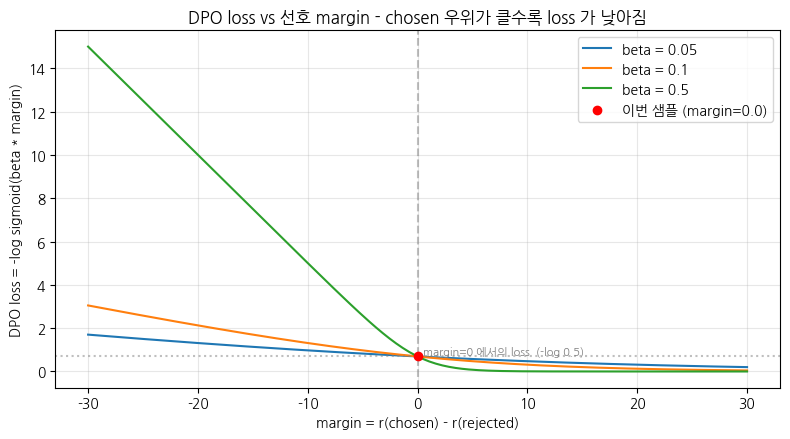
\includegraphics[width=0.86\linewidth]{assets/figures/ch30_dpo_loss_margin.png}
\end{bookfigurelabel}

\textbf{그림 읽기} --- 그림~\ref{fig:ch30-dpo-loss-margin}에서 다음 내용을 확인합니다: DPO loss와 preference margin의 관계. 실행된 노트북에서 저장된 최신 plot 출력이므로, 코드에서 계산한 값이 어떤 평가 지점으로 이어지는지 바로 확인할 수 있습니다.



\section{\texorpdfstring{\inlinecode{DPOTrainer} 로 DPO 학습 --- \emph{새 trainer, preference 정렬}}{DPOTrainer 로 DPO 학습 --- 새 trainer, preference 정렬}}

\inlinecode{trl.DPOTrainer} 는 본 장에 처음 등장합니다. §3 에서 손으로 한 \emph{response-only log-prob \(\to\) implicit reward \(\to\) margin \(\to\) sigmoid loss} 를 \emph{매 step 자동} 으로 수행합니다. 설정은 \inlinecode{DPOConfig} (\inlinecode{TrainingArguments} 상속) 로 주며, \textbf{\inlinecode{beta}} 가 reference 제약 강도입니다.

\begin{quote}
\textbf{VRAM 주의}: DPO 는 \emph{policy + frozen reference 두 모델} 을 메모리에 올립니다 (SFT 의 약 2배). T4 (16GB) 에서는 \textbf{batch 를 작게 (2) + gradient accumulation (8)} 으로 effective batch 16 을 만들고 \inlinecode{fp16=True} 로 메모리를 아낍니다. \inlinecode{ref\_model=None} 으로 주면 \inlinecode{DPOTrainer} 가 reference 를 자동 생성·freeze 합니다.
\end{quote}



\Needspace{11\baselineskip}
\begin{lstlisting}
from trl import DPOTrainer, DPOConfig

@torch.no_grad()
def reward_margins(model, ref, dataset, n=64):
    '''dataset 일부에 대해 implicit reward margin (chosen-rejected) 분포를 계산.'''
    model.eval()
    out = []
    for ex in dataset.select(range(min(n, len(dataset)))):
        pw = response_logprob(
            model,
            ex["prompt"],
            ex["chosen"],
        )
        pl = response_logprob(
            model,
            ex["prompt"],
\end{lstlisting}

\noindent\emph{앞 블록은 필요한 라이브러리와 기본 설정을 준비하는 단계입니다. 이어지는 블록에서는 앞에서 만든 중간 값을 다음 계산으로 넘기는 단계로 넘어갑니다.}

\Needspace{11\baselineskip}
\begin{lstlisting}[firstnumber=17]
            ex["rejected"],
        )
        rw = response_logprob(
            ref,
            ex["prompt"],
            ex["chosen"],
        )
        rl = response_logprob(
            ref,
            ex["prompt"],
            ex["rejected"],
        )
        out.append((pw - rw) - (pl - rl))
    return np.array(out)

\end{lstlisting}

\noindent\emph{앞뒤 블록은 모두 앞에서 만든 중간 값을 다음 계산으로 넘기는 단계입니다. 길이를 나누어 같은 흐름을 단계별로 확인합니다.}

\Needspace{11\baselineskip}
\begin{lstlisting}[firstnumber=32]
before_margins = reward_margins(
    policy,
    ref_model,
    dpo_ds,
    n=64,
)
acc_before = float((before_margins > 0).mean() + 0.5 * (before_margins == 0).mean())
print(
    f"BEFORE DPO - reward margin (n="
    f"{len(before_margins)})"
)
print(f"  mean margin     : {before_margins.mean():.3f}")
print(
    f"  reward accuracy : "
    f"{acc_before:.3f}  (ratio of margin>0; policy=ref 라 margin=0 -> 무승부 50%)"
)
\end{lstlisting}

\noindent\textbf{출력.}
\begin{bookoutputbox}
BEFORE DPO - reward margin (n=64)
  mean margin     : 0.000
reward accuracy : 0.500 (ratio of margin>0; policy=ref 라 margin=0 → 무승...
\end{bookoutputbox}
\par\vspace{0.9em}



\Needspace{11\baselineskip}
\begin{lstlisting}
dpo_config = DPOConfig(
    output_dir="./out_kogpt2_dpo",
    num_train_epochs=1,
    per_device_train_batch_size=2,
    gradient_accumulation_steps=8,
    # effective batch = 16
    learning_rate=5e-6,
    weight_decay=0.0,
    warmup_ratio=0.1,
    lr_scheduler_type="cosine",
    max_grad_norm=1.0,
    beta=BETA,
    max_length=512,
    fp16=USE_FP16,
    logging_steps=10,
    save_strategy="no",
\end{lstlisting}

\noindent\emph{앞 블록은 앞에서 만든 중간 값을 다음 계산으로 넘기는 단계입니다. 이어지는 블록에서는 학습 설정을 만들고 학습 루프를 실행하는 단계로 넘어갑니다.}

\Needspace{11\baselineskip}
\begin{lstlisting}[firstnumber=17]
    report_to="none",
    dataloader_num_workers=2,
    seed=SEED,
)

class VRAMCallback(__import__("transformers").TrainerCallback):
    '''step 별 peak VRAM 기록 (로깅 윈도우 단위 reset). CUDA 에서만 유효.'''

    def __init__(self):
        self.steps, self.peak_MiB = [], []

    def on_train_begin(self, args, state, control, **kwargs):
        if torch.cuda.is_available():
            torch.cuda.reset_peak_memory_stats()

\end{lstlisting}

\noindent\emph{앞 블록은 학습 설정을 만들고 학습 루프를 실행하는 단계입니다. 이어지는 블록에서는 앞에서 만든 중간 값을 다음 계산으로 넘기는 단계로 넘어갑니다.}

\Needspace{10\baselineskip}
\begin{lstlisting}[firstnumber=32]
    def on_log(self, args, state, control, logs=None, **kwargs):
        if torch.cuda.is_available():
            peak = torch.cuda.max_memory_allocated() / 1024**2
            self.steps.append(state.global_step)
            self.peak_MiB.append(peak)
            torch.cuda.reset_peak_memory_stats()

vram_cb = VRAMCallback()

\end{lstlisting}

\noindent\emph{앞 블록은 앞에서 만든 중간 값을 다음 계산으로 넘기는 단계입니다. 이어지는 블록에서는 텍스트를 모델 입력 텐서로 바꾸는 단계로 넘어갑니다.}

\Needspace{11\baselineskip}
\begin{lstlisting}[firstnumber=41]
trainer = DPOTrainer(
    model=policy,
    ref_model=None,
    args=dpo_config,
    train_dataset=dpo_ds,
    processing_class=tokenizer,
    callbacks=[vram_cb],
)

t0 = time.time()
train_out = trainer.train()
elapsed = time.time() - t0

\end{lstlisting}

\noindent\emph{앞 블록은 텍스트를 모델 입력 텐서로 바꾸는 단계입니다. 이어지는 블록에서는 앞에서 만든 중간 값을 다음 계산으로 넘기는 단계로 넘어갑니다.}

\Needspace{11\baselineskip}
\begin{lstlisting}[firstnumber=54]
print(f"\n=== DPO summary ===")
print(f"elapsed     : {elapsed/60:.2f} min")
print(f"global_step : {train_out.global_step}")
print(f"train_loss  : {train_out.training_loss:.4f}")
if torch.cuda.is_available():
    print(
        f"final peak  : "
        f"{torch.cuda.max_memory_allocated()/1024**2:.0f} MiB"
    )
\end{lstlisting}

\noindent\textbf{출력.}
\begin{bookoutputbox}
[transformers] warmup_ratio is deprecated and will be removed in v5.2. Use...
Key                                     | Status     |  | 
----------------------------------------+------------+--+-

[transformers] The tokenizer has new PAD/BOS/EOS tokens that differ from th...
Step  Training Loss
----  -------------
10    0.688411
20    0.710073
30    0.678711
40    0.817179
50    0.708727
60    0.683510
70    0.762712
80    0.680615
90    0.670623
...
\end{bookoutputbox}
\par\vspace{0.9em}



\section{\texorpdfstring{DPO 전·후 reward margin 비교 --- \emph{선호가 정렬됐는가}}{DPO 전·후 reward margin 비교 --- 선호가 정렬됐는가}}

본 장의 핵심 데모. \emph{같은 preference 샘플들} 에 대해 \emph{DPO 전} 과 \emph{DPO 후} 의 \textbf{reward margin (chosen - rejected 의 implicit reward)} 분포를 비교합니다.

\begin{itemize}
\tightlist
\item
  \textbf{DPO 전}: policy = reference \(\to\) margin 이 \emph{정확히 0} (무승부). reward accuracy 0.500
\item
  \textbf{DPO 후}: policy 가 \emph{chosen 을 더 선호} \(\to\) margin 분포가 \emph{양수 쪽으로 이동}, reward accuracy ↑
\end{itemize}

margin 분포가 \emph{오른쪽 (양수) 으로 밀려났다면} 정렬이 일어난 직접 증거입니다.

\begin{quote}
\textbf{측정 노트.} 학습 전에는 policy 와 reference 가 같아 margin 이 \emph{모든 샘플에서 정확히 0} 입니다. \textquotesingle margin\textgreater0 비율\textquotesingle{} 로만 세면 0.000 이 나오지만, 무승부(margin=0)는 동전 던지기처럼 50\% 이므로 \textbf{0.5 로 집계} 합니다 (코드의 \inlinecode{+\ 0.5\ *\ (margin\ ==\ 0)}). 그래야 before 0.500 \(\to\) after 0.844 로 정렬 효과가 왜곡 없이 읽힙니다.
\end{quote}



\Needspace{11\baselineskip}
\begin{lstlisting}
after_margins = reward_margins(
    policy,
    ref_model,
    dpo_ds,
    n=64,
)
acc_after = float((after_margins > 0).mean() + 0.5 * (after_margins == 0).mean())

print(
    f"AFTER DPO - reward margin (n="
    f"{len(after_margins)})"
)
print(
    f"  mean margin     : {after_margins.mean():.3f}  (before: "
    f"{before_margins.mean():.3f})"
)
\end{lstlisting}

\noindent\emph{앞 블록은 앞에서 만든 중간 값을 다음 계산으로 넘기는 단계입니다. 이어지는 블록에서는 숫자 결과를 그림으로 확인하는 단계로 넘어갑니다.}

\Needspace{11\baselineskip}
\begin{lstlisting}[firstnumber=17]
print(
    f"  reward accuracy : {acc_after:.3f}  (before: "
    f"{acc_before:.3f})"
)

fig, ax = plt.subplots(figsize=(8, 4.5))
bins = np.linspace(min(before_margins.min(), after_margins.min()),
                   max(
                       before_margins.max(),
                       after_margins.max()),
                       30,
                   )
ax.hist(before_margins, bins=bins, alpha=0.6, color="tab:gray",
        label=f"DPO 전 (acc={acc_before:.2f})")
ax.hist(after_margins, bins=bins, alpha=0.6, color="tab:green",
        label=f"DPO 후 (acc={acc_after:.2f})")
\end{lstlisting}

\noindent\emph{앞뒤 블록은 모두 숫자 결과를 그림으로 확인하는 단계입니다. 길이를 나누어 같은 흐름을 단계별로 확인합니다.}

\Needspace{11\baselineskip}
\begin{lstlisting}[firstnumber=33]
ax.axvline(
    0,
    color="red",
    ls="--",
    alpha=0.7,
    label="margin = 0",
)
ax.set_xlabel("reward margin = r(chosen) - r(rejected)")
ax.set_ylabel("개수")
ax.set_title("DPO 전 vs 후 - margin 이 양수 쪽으로 이동 (chosen 선호)")
ax.legend(); ax.grid(True, alpha=0.3)
plt.tight_layout(); plt.show()
\end{lstlisting}

\noindent\textbf{출력.}
\begin{bookoutputbox}
AFTER DPO - reward margin (n=64)
  mean margin     : 12.712  (before: 0.000)
  reward accuracy : 0.844  (before: 0.500)
\end{bookoutputbox}
\par\vspace{0.9em}

\begin{bookfigurelabel}[H]{DPO 전후 reward margin 분포 비교}{fig:ch30-dpo-margin-shift}
\centering
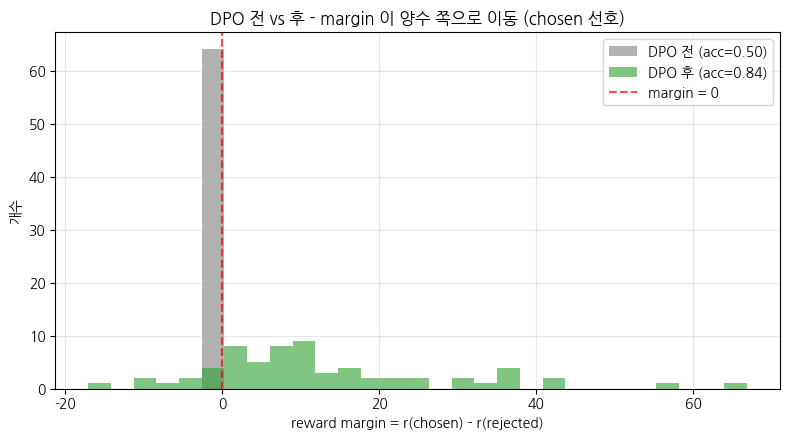
\includegraphics[width=0.86\linewidth]{assets/figures/ch30_dpo_margin_shift.png}
\end{bookfigurelabel}

\textbf{그림 읽기} --- 그림~\ref{fig:ch30-dpo-margin-shift}에서 다음 내용을 확인합니다: DPO 전후 reward margin 분포 비교. 실행된 노트북에서 저장된 최신 plot 출력이므로, 코드에서 계산한 값이 어떤 평가 지점으로 이어지는지 바로 확인할 수 있습니다.



\textbf{해석 가이드 --- preference alignment 의 증거}

\begin{itemize}
\tightlist
\item
  \textbf{before (gray)}: policy 가 아직 reference 와 같아 margin 이 \emph{0 근처에 모여} 있습니다. chosen 과 rejected 를 \emph{구별하지 못함} (reward accuracy \(\approx\) 0.5)
\item
  \textbf{after (green)}: 분포가 \emph{양수 쪽으로 이동} --- policy 가 \emph{chosen 의 implicit reward 를 rejected 보다 높게} 매깁니다. reward accuracy 가 0.5 보다 위로 올라갑니다
\end{itemize}

\begin{quote}
\textbf{핵심}: DPO 는 \emph{답변을 새로 생성하지 않고도}, \emph{주어진 (chosen, rejected) 쌍의 상대적 선호} 를 policy 에 새깁니다. 그게 \emph{implicit reward margin 의 양수 이동} 으로 나타납니다. KoGPT2 (125M) + 짧은 학습이라 이동 폭은 작을 수 있지만, \emph{방향} 이 양수로 잡혔다면 DPO 의 핵심 (선호 정렬) 은 작동한 것입니다.
\end{quote}

\begin{quote}
주의 KoGPT2 는 작은 base 모델이고 (정석은 SFT 모델에서 출발), DPO 데이터·시간도 작아 효과가 \emph{미묘} 할 수 있습니다. 관전 포인트는 \emph{생성 품질의 극적 향상} 이 아니라 \emph{\textbf{reward margin 이 chosen 쪽으로 이동했는가}} 입니다. 품질은 \emph{SFT 모델에서 출발 + 더 많은 preference + 더 큰 모델} 로 끌어올립니다 (FAQ 참고).
\end{quote}



\section{학습 곡선 --- DPO loss / reward 지표}

\inlinecode{DPOTrainer} 는 학습 중 \emph{loss} 뿐 아니라 \emph{reward margin·reward accuracy} 같은 DPO 고유 지표를 로깅합니다 (\inlinecode{trainer.state.log\_history}). loss 가 내려가고 reward accuracy 가 올라가는지 확인합니다.



\Needspace{11\baselineskip}
\begin{lstlisting}
log = trainer.state.log_history
steps = [r["step"] for r in log if "loss" in r]
losses = [r["loss"] for r in log if "loss" in r]

acc_key = "rewards/accuracies"
mgn_key = "rewards/margins"
accs = [(r["step"], r[acc_key]) for r in log if acc_key in r]
mgns = [(r["step"], r[mgn_key]) for r in log if mgn_key in r]

fig, (ax1, ax2) = plt.subplots(1, 2, figsize=(13, 4))

\end{lstlisting}

\noindent\emph{앞 블록은 학습 설정을 만들고 학습 루프를 실행하는 단계입니다. 이어지는 블록에서는 앞에서 만든 중간 값을 다음 계산으로 넘기는 단계로 넘어갑니다.}

\Needspace{11\baselineskip}
\begin{lstlisting}[firstnumber=12]
ax1.plot(
    steps,
    losses,
    "-",
    color="tab:blue",
    alpha=0.8,
    label="DPO loss",
)
ax1.set_xlabel("step"); ax1.set_ylabel("DPO sigmoid loss")
ax1.set_title("KoGPT2 DPO - loss")
ax1.grid(True, alpha=0.3); ax1.legend()

\end{lstlisting}

\noindent\emph{앞 블록은 앞에서 만든 중간 값을 다음 계산으로 넘기는 단계입니다. 이어지는 블록에서는 숫자 결과를 그림으로 확인하는 단계로 넘어갑니다.}

\Needspace{11\baselineskip}
\begin{lstlisting}[firstnumber=24]
if accs:
    ax2.plot([s for s, _ in accs], [a for _, a in accs], "o-",
             color="tab:green", label="reward accuracy")
if mgns:
    ax2b = ax2.twinx()
    ax2b.plot([s for s, _ in mgns], [m for _, m in mgns], "s--",
              color="tab:orange", alpha=0.7, label="reward margin")
    ax2b.set_ylabel("reward margin", color="tab:orange")
ax2.axhline(0.5, color="gray", ls=":", alpha=0.6)
ax2.set_xlabel("step"); ax2.set_ylabel("reward accuracy", color="tab:green")
ax2.set_title("DPO reward accuracy / margin  (chosen > rejected 비율)")
ax2.grid(True, alpha=0.3)

plt.tight_layout(); plt.show()

\end{lstlisting}

\noindent\emph{앞 블록은 숫자 결과를 그림으로 확인하는 단계입니다. 이어지는 블록에서는 앞에서 만든 중간 값을 다음 계산으로 넘기는 단계로 넘어갑니다.}

\Needspace{10\baselineskip}
\begin{lstlisting}[firstnumber=39]
if torch.cuda.is_available() and vram_cb.steps:
    print(f"peak VRAM (max over training): {max(vram_cb.peak_MiB):.0f} MiB"
          f"  (
              policy + reference,
              bs=2,
              grad_accum=8,
              fp16)",
          )
\end{lstlisting}

\noindent\textbf{출력.}
\begin{bookoutputbox}
peak VRAM (max over training): 4332 MiB (policy + reference, bs=2, grad_acc...
\end{bookoutputbox}
\par\vspace{0.9em}

\begin{bookfigurelabel}[H]{KoGPT2 DPO 학습 곡선과 reward 지표}{fig:ch30-dpo-training-curves}
\centering
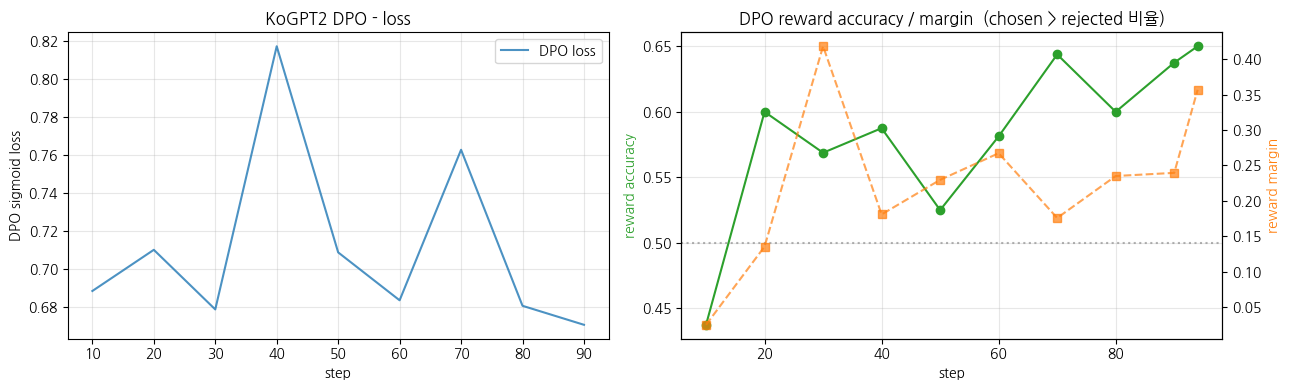
\includegraphics[width=0.90\linewidth]{assets/figures/ch30_dpo_training_curves.png}
\end{bookfigurelabel}

\textbf{그림 읽기} --- 그림~\ref{fig:ch30-dpo-training-curves}에서 다음 내용을 확인합니다: KoGPT2 DPO 학습 곡선과 reward 지표. 실행된 노트북에서 저장된 최신 plot 출력이므로, 코드에서 계산한 값이 어떤 평가 지점으로 이어지는지 바로 확인할 수 있습니다.



\section{\texorpdfstring{변형: \(\beta\) 조정 / 더 많은 preference / DPO 변종}{변형: \textbackslash beta 조정 / 더 많은 preference / DPO 변종}}

본 장에서 다루지 못한 변형들 --- 직접 시도해 보고 싶다면 아래를 출발점으로:

\subsection{\texorpdfstring{변형 1. \(\beta\) 조정 --- reference 제약 강도}{변형 1. \textbackslash beta 조정 --- reference 제약 강도}}

\Needspace{5\baselineskip}
\begin{lstlisting}

\end{lstlisting}

\subsection{변형 2. 더 많은 preference / SFT 모델에서 출발}

\Needspace{5\baselineskip}
\begin{lstlisting}

\end{lstlisting}

\subsection{변형 3. DPO 변종 --- IPO / KTO / ORPO}

\inlinecode{trl} 은 DPO 의 여러 변종을 \inlinecode{loss\_type} 으로 지원합니다:

\Needspace{5\baselineskip}
\begin{lstlisting}

\end{lstlisting}

\begin{quote}
IPO 는 \emph{DPO 의 overfitting} 을, KTO 는 \emph{쌍이 아닌 개별 좋음/나쁨 라벨} 을, ORPO 는 \emph{reference 없이 SFT 와 동시} 정렬을 노립니다. 모두 \emph{preference 로 정렬} 한다는 점은 같고, \emph{loss 형태·데이터 요구} 만 다릅니다.
\end{quote}



\section{이 장에 등장한 라이브러리·함수}

\begin{booktable}{30장 새로 등장한 라이브러리}{tab:ch30-09}
\begin{adjustbox}{max width=\textwidth}
\begin{tabular}{@{}lll@{}}
\toprule
이름 & 한 줄 설명 & \ref{ch:28}장과 차이 \\
\midrule

\inlinecode{trl.DPOTrainer} & DPO 특화 trainer (response-only log-prob \(\to\) margin \(\to\) sigmoid loss 자동) & \textbf{새로 등장} (\ref{ch:28}장 은 \inlinecode{SFTTrainer}) \\
\inlinecode{trl.DPOConfig} & \inlinecode{DPOTrainer} 설정 (\inlinecode{TrainingArguments} 상속 + \inlinecode{beta}·\inlinecode{max\_length} 등) & \textbf{새로 등장} \\
\inlinecode{DPOConfig(beta=0.1)} & reference 제약 강도 (KL) --- DPO 의 핵심 하이퍼파라미터 & \textbf{새로 등장} \\
\inlinecode{DPOTrainer(ref\_model=None)} & reference 자동 복사·freeze (명시 지정도 가능) & \textbf{새로 등장} (frozen reference 개념) \\
\inlinecode{prompt} / \inlinecode{chosen} / \inlinecode{rejected} 데이터 형식 & preference 쌍 표준 형식 & \textbf{새로 등장} (\ref{ch:28}장 은 \inlinecode{prompt}/\inlinecode{completion}) \\
\inlinecode{torch.nn.functional.log\_softmax} + \inlinecode{gather} & response 토큰의 log-prob 합 (§3 손계산) & \textbf{공유} (개념은 CausalLM loss 와 동일) \\
\inlinecode{copy.deepcopy(policy)} + \inlinecode{requires\_grad\_(False)} & frozen reference 직접 생성 (§3 시연용) & \textbf{새로 등장} \\
\inlinecode{PreTrainedTokenizerFast.from\_pretrained("skt/kogpt2-base-v2",\ ...)} & KoGPT2 BBPE (AutoTokenizer 함정 회피) & \textbf{공유} (\ref{ch:27}장 이후 고정) \\
\bottomrule
\end{tabular}
\end{adjustbox}
\end{booktable}

\begin{quote}
\inlinecode{trl} 은 버전마다 \inlinecode{DPOTrainer} / \inlinecode{DPOConfig} API 변동이 큽니다 (\inlinecode{max\_prompt\_length} 같은 인자가 버전에 따라 사라지기도). 본 노트북은 \emph{버전 간 안정적인 핵심 경로} (\inlinecode{prompt}/\inlinecode{chosen}/\inlinecode{rejected} 데이터 + \inlinecode{beta} + \inlinecode{max\_length} + \inlinecode{ref\_model=None}) 만 사용합니다. 설치된 \inlinecode{trl} 버전은 셋업 셀 출력에서 확인하세요.
\end{quote}



\section{체크포인트 질문}

\begin{enumerate}
\def\labelenumi{\arabic{enumi}.}
\tightlist
\item
  DPO 에서 \emph{왜 frozen reference 가 필요한가요?} reference 없이 (또는 \(\beta\)=0 으로) chosen 의 확률만 무한정 올리면 어떤 문제가 생기나요?
\item
  \emph{DPO 와 PPO (RLHF)} 는 둘 다 preference 로 정렬합니다. 그런데 DPO 가 \emph{T4 한 장에서 가능} 한 이유는 무엇인가요? (필요한 모델 개수로 설명)
\item
  DPO loss 의 \textbf{\(\beta\)} 가 \emph{크면} / \emph{작으면} 각각 어떤 trade-off 가 있나요? (정렬 속도 vs reference 에서 벗어남)
\item
  preference 데이터 \inlinecode{(prompt,\ chosen,\ rejected)} 는 어떻게 만드나요? 공개 데이터셋 외에, SFT 모델로 \emph{직접} 만들려면 어떤 절차가 필요할까요?
\end{enumerate}



\section{FAQ}

\begin{faqBox}{Q1. (이론) DPO 와 RLHF (PPO) 는 정확히 뭐가 다른가요?}

둘 다 \emph{preference 로 모델을 정렬} 하지만, \emph{경로} 가 다릅니다:

\begin{booktable}{30장 FAQ 표}{tab:ch30-10}
\begin{adjustbox}{max width=\textwidth}
\begin{tabular}{@{}lll@{}}
\toprule
항목 & PPO (RLHF) & DPO \\
\midrule

reward model & \emph{별도로 학습} (preference \(\to\) 점수 모델) & \textbf{없음} (preference 에서 직접) \\
학습 방식 & 강화학습 (rollout + advantage + PPO clip) & \textbf{지도학습} (loss.backward()) \\
필요 모델 & actor + critic + reward + reference (4개) & \textbf{policy + reference (2개)} \\
안정성 & RL 특유의 불안정 (튜닝 까다로움) & \textbf{상대적으로 안정} \\
\bottomrule
\end{tabular}
\end{adjustbox}
\end{booktable}

DPO 의 통찰은 \emph{“reward model 의 최적 정책을 닫힌 형태로 풀면, reward model 을 명시적으로 만들 필요 없이 preference 만으로 policy 를 직접 최적화할 수 있다”} 는 것입니다. 그래서 \emph{RM 학습 + RL 루프} 두 단계가 \emph{지도학습 한 단계} 로 줄어듭니다.

\Needspace{5\baselineskip}
\begin{lstlisting}

\end{lstlisting}

\end{faqBox}

\begin{faqBox}{Q2. (실무) reference 모델 없이 DPO 를 할 수 있나요?}

\inlinecode{DPOTrainer(ref\_model=None)} 은 \emph{reference 가 없는 게 아니라}, \emph{policy 의 복사본을 자동으로 reference 로 freeze} 하는 것입니다 (또는 PEFT 사용 시 adapter 를 끈 base 가 reference). 즉 reference 는 \emph{항상} 있습니다.

\emph{진짜로 reference 를 빼면} (\inlinecode{reference\_free} 류 옵션 또는 ORPO):

\begin{itemize}
\tightlist
\item
  KL 제약이 사라져 \emph{원본에서 멀어지는 것을 막을 닻이 없어집니다}
\item
  chosen 확률만 무한정 키우다 \emph{모델이 collapse (한 패턴 반복, 문법 collapse)} 할 위험
\item
  ORPO 는 \emph{reference 없이도} 작동하도록 \emph{loss 를 다르게 설계} 한 변종 (SFT 와 preference 를 한 번에)
\end{itemize}

\Needspace{5\baselineskip}
\begin{lstlisting}
trainer = DPOTrainer(model=policy, ref_model=None, args=cfg,
                     train_dataset=dpo_ds, processing_class=tokenizer)
\end{lstlisting}

\end{faqBox}

\begin{faqBox}{Q3. (이론) \(\beta\) 가 너무 크면 / 너무 작으면 어떻게 되나요?}

\(\beta\) 는 \emph{reference 에서 벗어나는 정도} 를 제어합니다 (KL 제약의 세기):

\begin{itemize}
\tightlist
\item
  \textbf{\(\beta\) 너무 큼} (예: 1.0): reference 제약이 \emph{거의 없음} \(\to\) policy 가 preference 에 강하게 끌려가 \emph{빨리 정렬} 되지만, \emph{원본 SFT 의 일반 능력이 collapse} (degeneration)·\emph{reward hacking} 위험. margin 만 키우려고 \emph{답변 품질을 희생} 할 수 있습니다
\item
  \textbf{\(\beta\) 너무 작음} (예: 0.01): reference 제약이 \emph{매우 강함} \(\to\) policy 가 reference 근처에 묶여 \emph{거의 안 움직임} \(\to\) 정렬이 느리거나 안 됨
\end{itemize}

\Needspace{5\baselineskip}
\begin{lstlisting}
dpo_config.beta = 0.1
\end{lstlisting}

\begin{quote}
직관: \(\beta\) 는 \emph{“preference 를 얼마나 공격적으로 따를 것인가 vs 원본을 얼마나 지킬 것인가”} 의 다이얼입니다.
\end{quote}

\end{faqBox}

\begin{faqBox}{Q4. (실무) preference 데이터 \inlinecode{(chosen,\ rejected)} 는 어디서 / 어떻게 만드나요?}

세 가지 경로:

\begin{enumerate}
\def\labelenumi{\arabic{enumi}.}
\tightlist
\item
  \textbf{공개 데이터셋}: 본 장의 \inlinecode{maywell/ko\_Ultrafeedback\_binarized}, 영어는 \inlinecode{Anthropic/hh-rlhf}, \inlinecode{argilla/ultrafeedback-binarized-preferences} 등
\item
  \textbf{사람 라벨링}: 같은 prompt 에 \emph{여러 답변} 을 생성 \(\to\) 사람이 \emph{더 나은 쪽을 chosen} 으로 표시 (RLHF 의 원형)
\item
  \textbf{AI 라벨링 (RLAIF)}: 강한 모델 (예: GPT-4) 이 \emph{어느 답이 더 나은지 판정} \(\to\) chosen/rejected 자동 생성
\end{enumerate}

\Needspace{5\baselineskip}
\begin{lstlisting}

\end{lstlisting}

핵심은 \emph{chosen 이 rejected 보다 “사람이 선호하는” 방향} 이면 된다는 점 --- 정답일 필요는 없고 \emph{상대적 선호} 만 있으면 DPO 가 작동합니다.

\end{faqBox}

\begin{faqBox}{Q5. (이론) DPO 변종 (IPO, KTO, ORPO) 은 무엇인가요?}

모두 \emph{preference 정렬} 의 변주입니다 --- \emph{loss 형태·데이터 요구} 만 다릅니다:

\begin{booktable}{30장 FAQ 표}{tab:ch30-11}
\begin{adjustbox}{max width=\textwidth}
\begin{tabular}{@{}lll@{}}
\toprule
변종 & 핵심 차이 & 언제 \\
\midrule

\textbf{IPO} & sigmoid 대신 \emph{squared loss} & DPO 의 \emph{overfitting} 완화 \\
\textbf{KTO} & \emph{쌍이 아닌} 개별 좋음/나쁨 라벨 & preference \emph{쌍을 만들기 어려울} 때 \\
\textbf{ORPO} & \emph{reference 없이} SFT + preference 동시 & reference 메모리 절약 + 단계 합치기 \\
\bottomrule
\end{tabular}
\end{adjustbox}
\end{booktable}

\Needspace{5\baselineskip}
\begin{lstlisting}
dpo_config.loss_type = "ipo"        # IPO
\end{lstlisting}

\begin{quote}
본 장은 \emph{원조 DPO (sigmoid loss)} 로 \emph{원리} 에 집중합니다. 변종들은 \emph{같은 목표 (chosen 선호 ↑), 다른 수단}.
\end{quote}

\end{faqBox}

\begin{faqBox}{Q6. (실무) 작은 모델 (KoGPT2 125M) DPO 의 한계는?}

DPO 의 효과는 \emph{출발 모델의 능력} 에 크게 의존합니다:

\begin{itemize}
\tightlist
\item
  \textbf{base 에서 출발 (본 노트북)}: 모델이 아직 \emph{지시를 잘 못 따르므로} preference 정렬 효과가 \emph{미묘}. 정석은 \emph{SFT 모델에서 출발}
\item
  \textbf{작은 모델}: chosen/rejected 의 log-prob 차이를 \emph{섬세하게} 다루기 어려워 margin 이동 폭이 작음
\item
  \textbf{짧은 학습}: 1 epoch / 1.5K 샘플은 \emph{방향} 을 보기엔 충분하지만 \emph{극적 변화} 는 어려움
\end{itemize}

\begin{quote}
본 장의 목표는 \emph{완성된 정렬 모델} 이 아니라 \emph{\textbf{DPO 가 무엇을 최적화하는가 (reward margin) 를 눈으로 확인}} 하는 것입니다. §3 의 손계산과 §5 의 margin 이동이 핵심. 실전 품질은 \emph{SFT 모델 + 큰 모델 + 많은 preference + LoRA} 의 영역.
\end{quote}

\end{faqBox}

\begin{faqBox}{Q7. (이론) 다음 단계 GRPO (\ref{ch:31}장) 는 DPO 와 뭐가 다른가요?}

둘 다 alignment (단계 4) 지만, \emph{선호의 출처} 가 다릅니다:

\begin{booktable}{30장 FAQ 표}{tab:ch30-12}
\begin{adjustbox}{max width=\textwidth}
\begin{tabular}{@{}lll@{}}
\toprule
단계 & 선호의 출처 & 데이터 \\
\midrule

\textbf{DPO (\ref{ch:30}장)} & \emph{사람이 비교} 한 preference 쌍 & \inlinecode{(prompt,\ chosen,\ rejected)} \\
\textbf{GRPO (\ref{ch:31}장)} & \emph{verifier 가 자동 채점} 한 reward & verifiable-reward prompts (수학·코드) \\
\bottomrule
\end{tabular}
\end{adjustbox}
\end{booktable}

\begin{quote}
DPO 는 \emph{주관적 선호} (어느 답이 더 좋은가 --- 사람 판단) 를, GRPO 는 \emph{객관적 정답} (수학 답이 맞나, 코드가 돌아가나 --- 자동 검증) 을 신호로 씁니다. GRPO 는 \emph{같은 prompt 에 여러 답을 rollout} 해 \emph{그룹 안에서 상대 비교} (group relative advantage) 합니다 --- \ref{ch:31}장에서 본격.
\end{quote}

\Needspace{5\baselineskip}
\begin{lstlisting}
# from trl import GRPOTrainer, GRPOConfig
\end{lstlisting}
\end{faqBox}



\begin{previewBox}{미리보기: 다음 장}

\textbf{\ref{ch:31}장. GRPO --- verifier reward 로 정렬 (Group Relative Policy Optimization)}

\begin{itemize}
\tightlist
\item
  DPO 는 \emph{사람이 비교한 preference 쌍} 으로 정렬했다면, GRPO 는 \emph{verifier 가 자동 채점한 reward} 로 정렬 --- 수학·코드처럼 \emph{정답을 자동 검증} 할 수 있는 영역
\item
  \emph{같은 prompt 에 여러 답을 rollout} \(\to\) \emph{그룹 안에서 상대 비교} (group relative advantage) \(\to\) reward 높은 답 쪽으로 정책 강화
\item
  reward model 도, critic 도 없이 \emph{그룹 평균을 baseline} 으로 advantage 를 만드는 \emph{PPO 의 또 다른 간소화}
\item
  alignment 의 \emph{두 방식 비교}: \textbf{DPO (주관적 선호, 사람 비교) vs GRPO (객관적 정답, 자동 검증)}
\end{itemize}

\textbf{Phase 4 GPT 시대 4단계 흐름 정리}:

\begin{booktable}{30장 FAQ 표}{tab:ch30-13}
\begin{adjustbox}{max width=\textwidth}
\begin{tabular}{@{}lllll@{}}
\toprule
장 & 단계 & 본체 & 데이터 & 학습 신호 \\
\midrule

\ref{ch:24}·\ref{ch:26}장 & 1 (pretraining) & 작은 GPT scratch & TinyStories (영/한) & next-token \\
\ref{ch:25}·\ref{ch:27}장 & 2 (continual pretraining) & gpt2 / KoGPT2 & TinyStories (동일) & next-token \\
\ref{ch:28}장 & 3 (SFT) & KoGPT2 & KoAlpaca instruction-response & response 토큰 \\
\textbf{\ref{ch:30}장 \(\leftarrow\) 여기} & \textbf{4 (alignment, DPO)} & \textbf{SFT 모델 + frozen ref} & \textbf{preference 쌍 (chosen/rejected)} & \textbf{chosen 선호 ↑, rejected \(\downarrow\)} \\
\ref{ch:31}장 & 4 (alignment, GRPO) & SFT 모델 + verifier & verifiable-reward prompts & group relative advantage \\
\bottomrule
\end{tabular}
\end{adjustbox}
\end{booktable}

\begin{quote}
\textbf{변하는 축} (\ref{ch:28}장 \(\to\) \ref{ch:30}장): \emph{학습 단계} (SFT \(\to\) alignment). 본체·토크나이저는 SFT 모델을 잇고, \emph{데이터 (preference 쌍) + trainer (\inlinecode{DPOTrainer}) + loss (DPO sigmoid) + reference 모델} 이 바뀝니다. \inlinecode{labels\ =\ -100} 의 \emph{response-only} 원리는 DPO 의 log-prob 계산에서도 이어집니다 --- Phase 4 를 관통하는 thread.
\end{quote}
\end{previewBox}